% Template for ICASSP-2017 paper; to be used with:
%          spconf.sty  - ICASSP/ICIP LaTeX style file, and
%          IEEEbib.bst - IEEE bibliography style file.
% --------------------------------------------------------------------------
\documentclass{article}


\usepackage[final]{nips_2016}


\usepackage[utf8]{inputenc} % allow utf-8 input
\usepackage[T1]{fontenc}    % use 8-bit T1 fonts
\usepackage[draft]{hyperref}       % hyperlinks
\usepackage{url}            % simple URL typesetting
\usepackage{booktabs}       % professional-quality tables
\usepackage{amsfonts}       % blackboard math symbols
\usepackage{nicefrac}       % compact symbols for 1/2, etc.
\usepackage{microtype}      % microtypography

\usepackage{amsmath,graphicx}
\usepackage{bm}
\usepackage{url}
\usepackage{amsmath}
\usepackage{amsthm}
\usepackage{graphicx}
\usepackage{subcaption}
\usepackage{algorithm2e}
\usepackage{pbox}
\usepackage{multirow}

% Example definitions.
% --------------------
\def\x{{\mathbf x}}
\def\L{{\cal L}}

% Title.
% ------
\title{Invariant Representations for Noisy Speech Recognition}
%
% Single address.
% ---------------
%\name{Dmitriy Serdyuk $^{\dagger}$\thanks{Dmitriy Serdyuk performed the work
%  while at IBM}, Kartik Audhkhasi$^{\star}$, Phil\'emon Brakel$^{\dagger}$, Bhuvana Ramabhadran$^{\star}$, Yoshua Bengio$^{\dagger}$\thanks{Yoshua Bengio is a CIFAR Fellow.}}
%\address{$^{\dagger}$ Universit\'e de Montr\'eal\\
%         $^{\star}$ IBM}
\author{
  Dmitriy Serdyuk\thanks{Dmitriy Serdyuk performed the work 
    during an internship at IBM Watson} \\
  MILA\\
  Universit\'e de Montr\'eal\\
  Montr\'eal, QC H3T 1J4 \\
  \texttt{serdyuk@iro.umontreal.ca} \\
  \And
  Kartik Audhkhasi \\
  IBM Watson Research Center \\
  Yorktown Heights, NY 10598\\
  \texttt{kaudhkha@us.ibm.com} \\
  \And
  Phil\'emon Brakel \\
  MILA\\
  Universit\'e de Montr\'eal\\
  Montr\'eal, QC H3T 1J4 \\
  \texttt{pbpop3@gmail.com} \\
  \And
  Bhuvana Ramabhadran\\
  IBM  Watson Research Center\\
  Yorktown Heights, NY 10598\\
  \texttt{bhuvana@us.ibm.com} \\
  \And
  Samuel Thomas\\
  IBM  Watson Research Center\\
  Yorktown Heights, NY 10598\\
  \texttt{bhuvana@us.ibm.com} \\
  \And
  Yoshua Bengio\\
  MILA, CIFAR Fellow\\
  Universit\'e de Montr\'eal\\
  Montr\'eal, QC H3T 1J4 \\
  \texttt{findme@inter.net} \\
}



\begin{document}
%\ninept
%
\maketitle
%
\begin{abstract}
    Robustness of a speech recognition system is a challenging task and modern
    automatic speech recognition (ASR) systems need to be resilient to different recording conditions,
    microphone type, accents, and noisy recording environment. We mitigate
    this problem in a fashion similar to recent research on image generation using
    Generative Adversarial Networks and domain adaptation ideas extending
    adversarial gradient-based training. A recent work of Ganin et al. proposes to
    use adversarial training procedure for image domain adaptation making an intermediate
    representation to improve the target performance and at the same time
    to deteriorate the domain classifier performance, which is a separate neural
    network taking the intermediate representation as the input.
    This work focuses on investigation of neural architectures which produce
    representations invariant to certain conditions as the noise type for speech
    recognition. Similar
    to the Ganin et al. work we train the intermediate representation to be invariant
    to noise conditions training three neural networks: the encoder, the recognizer, and the
    noise classifier to produce the representation produced by the encoder to decrease
    the performance of the classifier making the representation invariant to noise conditions. We
    experimentally evaluate proposed architectures on the acoustic modelling task
    for speech recognition on a popular benchmark Aurora-4.
\end{abstract}
%
%\begin{keywords}
%speech recognition, deep neural networks, invariant representations, adversarial training
%\end{keywords}
%
\section{Introduction}
\label{sec:intro}
    One of the most challenging aspects of automatic speech recognition (ASR),
    is the mismatch between the training and testing conditions. During
    testing, a system may encounter new recording conditions, microphone types,
    accents and types of background noises. Even if all testing conditions also appeared
    in the train data, their relative distribution is likely to be
    different. For this reason, it's important to develop systems that are
    robust towards changes in recording conditions in general.

    While many types of model and feature based adaptation methods like MLLR and fMLLR
    \cite{leggetter1995maximum} have been proposed, most of these methods have
    been designed with GMM-HMM systems in mind. Since the enormous success of
    Deep Neural Network (DNN) systems for ASR \cite{hinton2012deep}, GMM-based
    model adaptation is not possible anymore, while feature-based methods may
    not be optimal anymore.
    Moreover, the discriminative gradient-based optimization used to train
    DNNs, in combination with the ability of DNNs to learn highly non-linear
    feature transformations, allows for more flexibility when it comes to the
    construction of training objectives that promote domain invariant
    representations.

    The main idea of this work is that instead of training a robust system,
    it is possible to train a system which will be invariant to these 
    conditions. This method of training requires the labels in the dataset
    which indicate which condition a particular recording was taken in, the 
    test data doesn't need to contain these labels. The method was proposed in
    the context of image classification in~\cite{ganin2014unsupervised} and 
    will be explained in Section~\ref{sec:gradient-reverse} and the application 
    to speech recognition is discussed
    in Section~\ref{sec:invariant-speech}. It is tightly connected to the idea
    of generative adversarial networks (GAN) proposed 
    in~\cite{goodfellow2014generative} thus we start with the discussion
    on this type of generative networks in Section~\ref{sec:gans}

    %TODO

\section{Generative Adversarial Networks}
\label{sec:gans}
    One of the most insightful recent advantages in the area of generative models
    is the models of the family of generative adversarial networks (GAN).
    A GAN consists of two networks: generator and discriminator. The generator 
    network $G$ has an
    input of randomly generated vector and is asked to produce an image 
    similar to the images in the training set. The discriminator network $D$
    can either receive a generated image from the generator $G$ or an image
    from the training set, the task of the discriminator is to distinguish
    between a generated image and a ``real'' image taken from the dataset. Thus
    the discriminator is just a classifier network with a sigmoid output
    and can be trained with the gradient methods. The main idea of the generative adversarial
    training is that it is possible to propagate the gradient of the discriminator
    network further to the generator network stacking them on top of each other.
    This leads to an efficient training procedure and GANs achieved the state of the
    art that time on handwritten digit generation MNIST dataset.

    In other words, these two networks are competing with each other the 
    generator is trying to deceive the discriminator network while it tries
    to do its best to recognize if there was a deception. This game theoretical
    similarity gave a name of adversarial networks. If we put it formally, the 
    objective of adversarial training is
    \begin{align*}
        \min_G \max_D V(D, G) = \mathbb{E}_{\bm{x} \sim p_{\text{data}}(\bm{x})}[\log D(\bm{x})] + 
            \mathbb{E}_{\bm{z} \sim p_{\bm{z}}(\bm{z})}[\log (1 - D(G(\bm{z})))].
    \end{align*}

    In practice, GANs might be hard to train due to the fact that in a case when 
    the discriminator is more powerful that the generator, the later doesn't 
    receive any gradient thus can not be improved. Usually this problem is solved
    using a smart schedule which stops learning the discriminator as soon as it
    is too far ahead of the generator. Other possible solutions include ``soft''
    targets bounded at some constant rather than between 0 and 1 and using a 
    different proxy for the cost.

\section{Gradient Reverse Method}
\label{sec:gradient-reverse}

    A work~\cite{ganin2014unsupervised} proposes a method of training a network 
    which can be adapted to new domains. The training set consists of the images
    labeled with classes and the separate domain labels. The test set doesn't need
    to have the domain labels. For example, it may be first domain
    consisting of MNIST digits and second domain of MNIST digits on a different
    background. The network has a fork-like structure: the image is fed to the
    first network which produces a hidden representation $h$, then there are two
    networks branching of the representation $h$: a domain classifier network and 
    a target classifier. The goal of the training is to produce the hidden 
    representation invariant to the domain labels so that information doesn't 
    interfere the target classifier which is used in the test time.

    The network is trained with three goals: the hidden representation $h$ should
    be helpful for the target classifier, but harmful for the domain classifier,
    the domain classifier should have a good classification accuracy. More 
    formally, we define the objective as
    \begin{equation}
        L = L(\hat{y}, y; \theta_R, \theta_E) + 
        \alpha L(\hat{d}, d; \theta_D) -
        \beta L(\hat{d}, d; \theta_E),
    \end{equation}
    where $y$ is the ground truth class, $d$ is the domain label, corresponding
    hatted variables are the network predictions, $\theta$ are the network 
    parameters, and $E, R, D$ are the subsets of parameters in the encoder,
    recogniser and the domain adaptation networks respectively. The hyper-parameters
    $\alpha$ and $\beta$ denote the influence of every part of the cost.

\subsection{Invariant Represenations for Speech Recognition}
\label{sec:invariant-speech}

In this work we focus on speech recognition using DNN-HMM hybrid systems. The
recording conditions, speaker identity, or gener might be considred to be domains
and adptation task corresponds to making the hidden layer representations be 
invariant with respect to those conditions. We hypothesize that this method of
training helps to generalize on unseen conditiions and requires only very small
amount of labeling the conditions, see Section~\ref{sec:experiments} for experimental
evaluation.

The model we use is depicted on Figure~\ref{fig:model}. It is a feedforward neural network
which is trained to predict the HMM state tweaked with a branch for the invariance
training. This branch is discarded in the testing phase. In our experiments we
used the noise condition as the domain label merging all noise type to one label
and clean type to another.

The particular cost we used for our training is
    \begin{equation}
        L = L_1(\hat{y}, y; \theta_R, \theta_E) + 
        L_2(\hat{d}, d; \theta_D) +
        \beta L_3(\hat{d}, d; \theta_E),
        \label{eq:cost}
    \end{equation}
where $L_3 = - d\log(1 - \hat{d}) - (1-d)\log(\hat{d})$ maximizes the probablity
of an incorrect domain classification. The terms for $L_1$ and $L_2$ are 
regular cross-entropy terms which are minimized with respect to the parameters
after semicolon.
We don't use any coefficient for first two terms because it is equivalent to 
changing the learning rate.


\begin{figure}
    \centering
    \captionsetup[subfigure]{oneside,margin={0.3cm,0cm}}
    \begin{subfigure}[b]{0.4\linewidth}
        \centering
        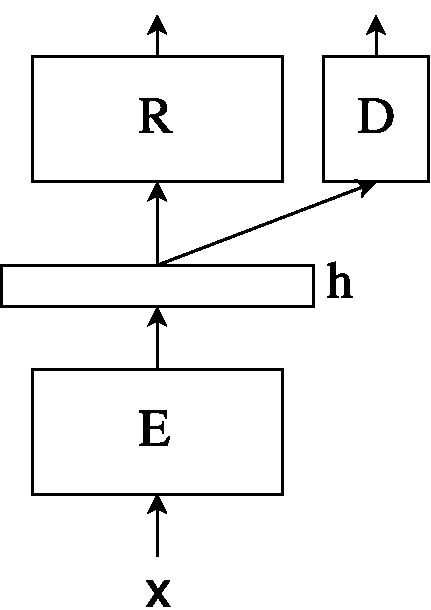
\includegraphics[width=0.9\linewidth]{model.pdf}
        \caption{The model consists of three neural networks. The encoder $E$ produces
        the intermediate representation $h$ which used in the recognizer $R$ and 
        in the discriminator $D$. The hidden representation $h$ is trained to improve
        the recognition and minimize the discrimination accuracy. The discriminator
        is a classifier trained to maximize its accuracy on the gender or the noise type
        recognition task.}
        \label{fig:model}
    \end{subfigure}%
    \begin{subfigure}[b]{0.6\linewidth}
        \centering
        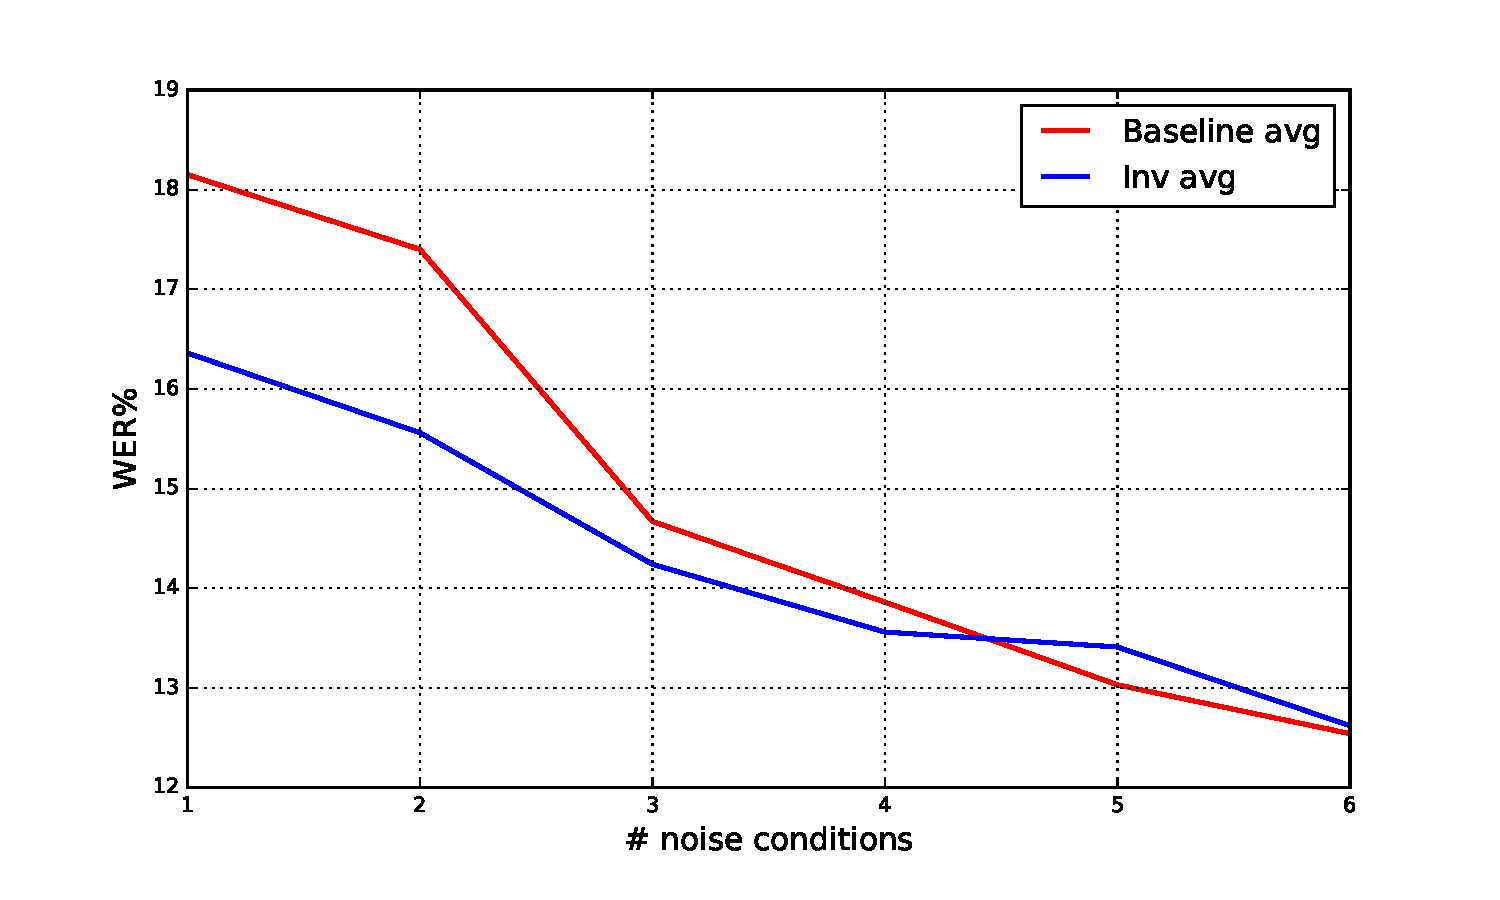
\includegraphics[width=\linewidth]{wer_avg.pdf}
        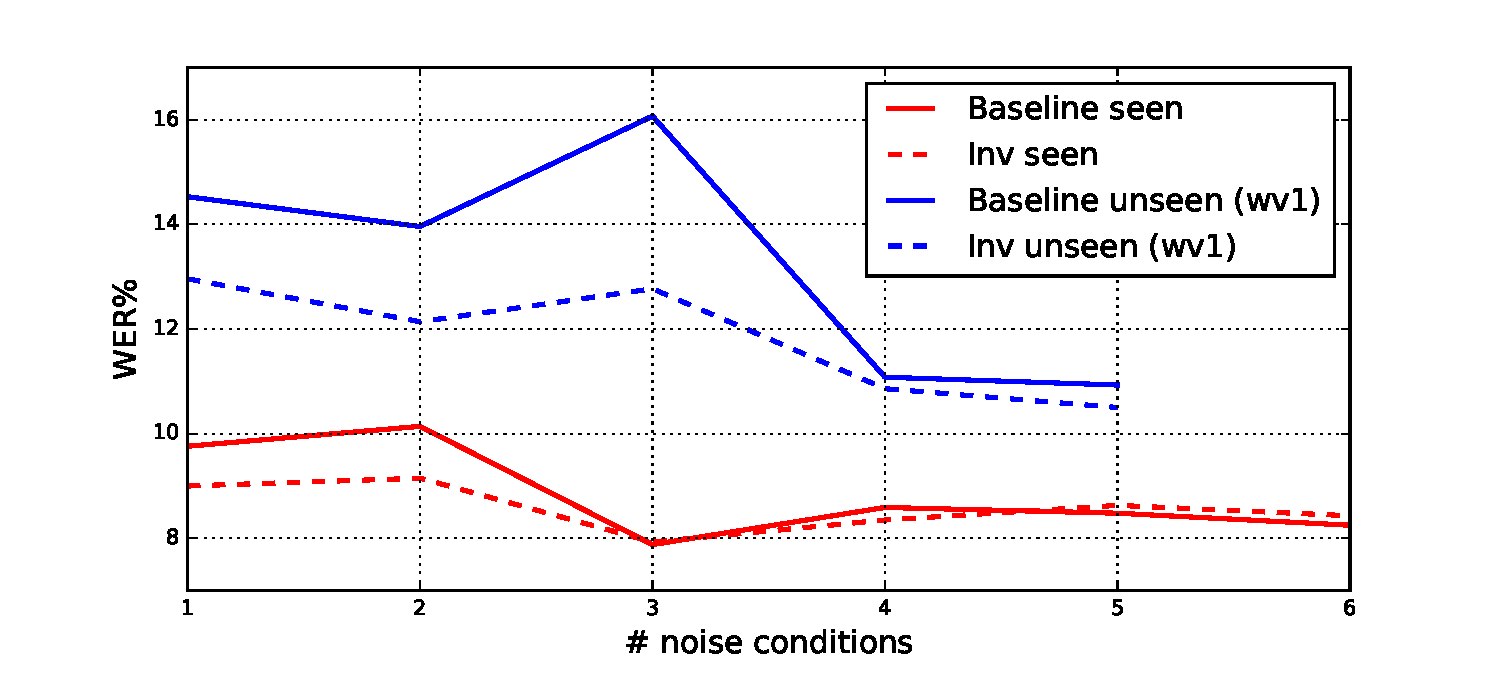
\includegraphics[width=\linewidth]{wer_seen_unseen.pdf}
        \caption{Up: Average performance of the model depending on the number of noise
            conditions used for training. Bottom: Average performance on seen condition versus unseen.
            Testing was performed on all wv1 conditions.
            }
        \label{fig:model}
    \end{subfigure}%
\end{figure}

\section{Related Work}
    Earlier approaches include various works on denoising including 

    In a work~\cite{yusuke2016adversarial} an acoustic model trained in an adversarial fashion is
    applied to an in-house dataset based on Wall Street Journal 1 corrupted with additive noise.
    

\section{Experiments}
\label{sec:experiments}
We experimentally evaluate the approach discussed in Section~\ref{sec:gradient-reverse} 
on a noisy speech recognition dataset Aurora-4~\cite{parihar2002aurora}. This dataset
is based on the Wall Street Journal corpus (WSJ0 is available at LDC). It contains noise of 
six categories which was added to clean
data. Every clean and noisy utterance filtered to simulate sampling frequency. The train
set contains approximately 4400 clean utterances and 446 utterances of each noise condition,
in total 2676 noisy utterances.
The test
set contains clean data, the same 6 noises, and data recorded with a different microphone
both clean and noise corrupted.

We used 16kHz training audio. We extracted mel-filterbank features with their deltas and 
delta-deltas spliced over 5 frames on each side making 11 consecutive frames and 1320 input 
features in total. Global mean and variance normalization was applied to these features.
We did not use any speaker normalization of input features. We trained 6 layer
speech recognition network with 2048 rectified linear units at every layer using momentum
accelerated stochastic gradient descent for 15 epochs. We annealed the learning rate accroding 
to the development set dividing it by 2 when the cross entropy did not improve.

In order to evaluate the impact of our method on generalization to new, unseen noises 
we performs 6 groups of experiments with different set of seen noises. We always train
on clean data and add noise conditions one-by-one in order: airport, babble, car, 
restaurant, street, train. The last group includes all noises therefore matches the
standard multi condition training setup. For every group of experiments we trained the
baseline and the invariance model where we branch out at 4th layer to a logistic 
binary classifier clean versus noisy data. Due to the imballance between clean and
noisy parts of the dataset, we had to oversample noisy frames, every minibatch contained
half of clean and half of noisy data points.

The results are summarized in Table~\ref{tab:results}. 
In our experiments we did not use layerwise pretraining not uncommonly used for small
datasets due to the difficulties of combining it with the invariance training. Our preliminary
experiments show that the network is not able to leave the parameter region it reaches after 
pretraining.

%\begin{figure}
%    \centering
%    \begin{subfigure}[b]{0.5\linewidth}
%        \centering
%        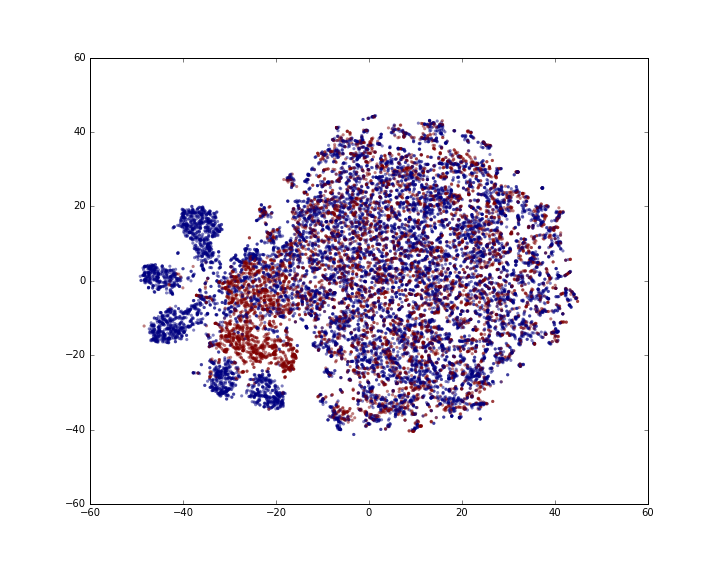
\includegraphics[width=\linewidth]{tsne-original.png}
%    \end{subfigure}%
%    \begin{subfigure}[b]{0.5\linewidth}
%        \centering
%        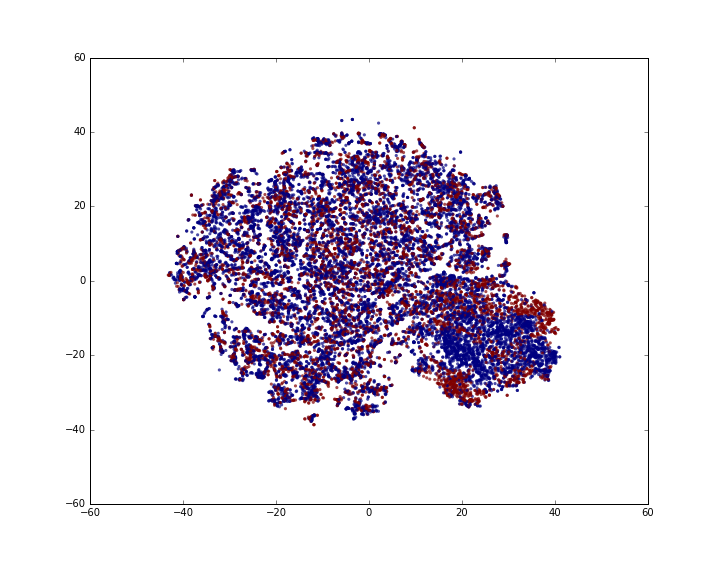
\includegraphics[width=\linewidth]{tsne-invariant.png}
%    \end{subfigure}%
%    \caption{t-SNE visualization of the last hidden layer using the clean development
%    subset. On the left, the baseline
%    model. On the right, the model trained with the adversarial objective. Colors 
%    represent genders.}
%    \label{fig:tsne}
%\end{figure}

\begin{table}
    \centering
    \caption{Average word error rate (WER\%) on Aurora-4 dataset on all test conditions,
        including seen and unseen noise and unseen microphone. First column
        is the number of noise conditions used for the training. The last row is a 
        preliminary experiment with layer-wise pretraining close to state-of-the-art
        model and a corresponding invariance training starting with a pretrained model.}
    \label{tab:results}
    \begin{tabular}{r|cc||cc|cc|cc|cc}
    %\multirow{2}{*}{Subset} & \multicolumn{2}{c}{Orig}  & \multicolumn{2}{|c}{Inv}\\ 
    %           & wv1  & wv2  & wv1  & wv2 \\
        Noise       &Inv&BL&  \multicolumn{2}{c|}{A} & \multicolumn{2}{c|}{B} & \multicolumn{2}{c|}{C} & \multicolumn{2}{c}{D}\\
               & & &  Inv & BL & Inv & BL & Inv & BL & Inv & BL\\
    \hline
    1           &16.36        &18.14 &6.54&7.57    &12.71& 14.09   & 11.45&   13.10    & 22.47 &   24.80    \\
    2           &15.56        &17.39 &5.90&  6.58 &   11.69   &13.28   &11.12   &13.51   &21.79   &23.96 \\
    3           &14.24        &14.67 &5.45 & 5.08&    10.76&   12.44&   9.75&    9.84 &   19.93&   19.30\\
    4           &13.61        &13.84 & 5.08 &5.29    &9.73    &9.97    &9.49    &9.56    &19.49   &19.90\\         
    5           &13.41        &13.02 & 5.12 &5.34    &9.52    &9.42    &9.55    &8.67    &19.33   &18.65\\         
    6           &12.62        &12.60 & 4.80 &4.61    &9.04    &8.86    &8.76    &8.59    &18.16   &18.21\\
    \hline\hline
    6* &11.88        &11.99
    \end{tabular}
    %TODO: add numbers!
\end{table}

\section{Discussion}
    We demonstrate that the invariance training helps to generalize to unseen noise
    conditions and improves in 
    
    The task of speech recognition differs from the image recognition
    adaptation in an aspect of the domain adaptation network training dynamics. 
    While the most common problem for the GAN type of networks trained on images 
    is overfitting, the noise type classification networks suffers from 
    underfitting. This makes the gradient of the $L_3$ term in Eq.~\ref{eq:cost}
    unrealiable and noisy. 


\section*{Acknowledgments}

We would like to thank Yaroslav Ganin, David Warde-Farley for insightful discussions,
developers of Theano~\cite{2016arXiv160502688short}, Blocks, and Fuel~\cite{MerrienboerBDSW15} 
for great instruments.

% References should be produced using the bibtex program from suitable
% BiBTeX files (here: strings, refs, manuals). The IEEEbib.bst bibliography
% style file from IEEE produces unsorted bibliography list.
% -------------------------------------------------------------------------
%\bibliographystyle{IEEE}
\bibliographystyle{authordate1}
\bibliography{refs}

\end{document}
